\documentclass[11pt]{article} % use larger type; default would be 10pt

% Common packages for mathematical articles
\usepackage{fullpage,amsmath,amsfonts,mathpazo,microtype,nicefrac,algorithm2e,graphicx}

% MSE Packages
\usepackage{caption}
\usepackage{physics}
\usepackage{xcolor}
\usepackage{listings}
\usepackage{parskip}
\usepackage{float}

% MSE Make margins a bit smaller
\usepackage[margin=0.75in]{geometry}
\usepackage[font=footnotesize]{caption}

% MSE set graphics path
\graphicspath{{../figs/}}

% Set-up for hypertext references
\usepackage{hyperref,color,textcomp}
\definecolor{webgreen}{rgb}{0,.35,0}
\definecolor{webbrown}{rgb}{.6,0,0}
\definecolor{RoyalBlue}{rgb}{0,0,0.9}
\hypersetup{
   colorlinks=true, linktocpage=true, pdfstartpage=3, pdfstartview=FitV,
   breaklinks=true, pdfpagemode=UseNone, pageanchor=true, pdfpagemode=UseOutlines,
   plainpages=false, bookmarksnumbered, bookmarksopen=true, bookmarksopenlevel=1,
   hypertexnames=true, pdfhighlight=/O,
   urlcolor=webbrown, linkcolor=RoyalBlue, citecolor=webgreen,
   pdfsubject={Harvard IACS AC 290 R},
   pdfkeywords={},
   pdfcreator={pdfLaTeX},
   pdfproducer={LaTeX with hyperref}
}
\hypersetup{pdftitle={AC290-RBC}}


% MSE Macros
\newcommand{\tty}[1]{\texttt{#1}}
\newcommand{\uu}{\vectorbold{u}}
\newcommand{\vv}{\vectorbold{u}}
\newcommand{\Laplace}{\Delta}
\renewcommand{\vec}[1]{\mathbf{#1}}

%***Start of Document***
\title{Hemodynamic Simulation with Lattice Boltzman}
\author{Harvard IACS AC 290R - Group 1 \\
Michael S. Emanuel \\
Jonathan Guillotte-Blouin \\
Yue Sun \\
}
\date{28-April-2019} 

\begin{document}
\maketitle

\section{Problem Statement and Motivation}
AC 290R is a course on extreme computing with a focus on the application domain of fluid dynamics.
In our first module we took on a prototypical problem using the continuum description of fluids
governed by the Navier-Stokes equation: 
\href{https://en.wikipedia.org/wiki/Rayleigh%E2%80%93B%C3%A9nard_convection}{Rayleigh-B\'enard Convection}.
In this module, we shift from the continuum to the mesoscale description and simulate fluids using  
\href{https://en.wikipedia.org/wiki/Lattice_Boltzmann_methods}{Lattice Boltzmann} methods.  
These methods are based on the Boltzmann Equation of thermodynamics and statistical physics.

The particular task we undertook was a hemodynamic simulation.
\href{https://en.wikipedia.org/wiki/Hemodynamics}{Hemodynamics} is the study of the dynamics of blood flow.  
It is a rich field at the intersection of anatomy and physics with a storied history.
Pioneers in the field include 
\href{https://en.wikipedia.org/wiki/Leonardo_da_Vinci}{Leonardo Da Vinci}, 
\href{https://en.wikipedia.org/wiki/Leonhard_Euler}{Leonhard Euler,} 
\href{https://en.wikipedia.org/wiki/Thomas_Young_(scientist)}{Thomas Young}, and 
\href{https://en.wikipedia.org/wiki/Jean_L%C3%A9onard_Marie_Poiseuille}{Jean L.M. Poieseuille}.

The particular problem was as follows.  
We aim to model the dispersion of a therapeutic drug that is injected with a catheter to treat a stenotic artery.
Stenosis is a disease of the arteries in which an artery becomes narrowed.
It is frequently caused by 
\href{https://en.wikipedia.org/wiki/Atherosclerosis}{atherosclerosis}, 
a build-up of fatty deposits (cholesterol) on the walls of the artery.
Stenotic arteries can cause serious medical problems including heart attacks and strokes.
One approach to treating stenoses is to introduce a therapeutic drug with a catheter,
a small tube inserted surgically into the patient that can be threaded through the circular system.
The goal of our simulation was to understand how the drug molecules dispersed 
and to see how many of them passed through the stenotic region, and at what times.

This is a worthwhile object of study for both pedagogical and practical reasons.
Pedagogically, this topic rounds out our survey of both techniques and domain knowledge in the course.
We are aiming to master the techniques of extreme computing and their application to fluid dynamics.
The first topic covered the continuum approach, and this topic covers the mesoscale approach.
The first topic used traditional CPU-centric computations, and this topic introduces us to GPU computing.

On a practical level, \href{https://www.cdc.gov/heartdisease/facts.htm}{heart disease} 
has been for many years a leading cause of death in Americans alongside cancer.
It is a complex disease with many treatment options and a need for accurate diagnosis.
Clinical practice still often relies on human judgment about which arterial blockages 
look risky, and there is reason for optimism that advances in biologically realistic computer
simulations could lead to materially faster and more accurate diagnosis 
and improve treatement selections.

\newpage
\section{Overview of Numerical Methods Used}
The main numerical method used in this simulation is the Lattice Boltzmann Method (LBM).
LBM is based on the \href{https://en.wikipedia.org/wiki/Boltzmann_equation}{Boltzmann Equation},
which describes the statistical behavior of a thermodynamic system and dates to 1872.
The idea behind the Boltzmann Equation is that particles in the system each have 6 degrees
of freedom, 3 positions and 3 momenta along the 3 coordinate directions $x$, $y$ and $z$.
Molecules of a given type are physically indistinguishable from each other,
so the system can be described completely by the populations of particles as a function
of time and these six dimensions in the phase space.
The Boltzmann Equation describes the evolution of such a system.
The populations of particles change due to three terms: 
diffusion, collisions, and external forces.

LBM is a technique in computational fluid dynamics that uses the Boltzmann Equation
to devise a numerical simulation of a fluid that can accurately capture mesoscale dynamics
when it is tuned properly.
The physical system is discretized, typically on a rectilinear grid 
and most commonly one with cubic spacing.  
Particle velocities are also discretized, with particles allowed to jump from one grid point only to nearby grid points over one simulation step.
The most common discretization scheme for 3D fluid simulations,
which we used for this problem, is called D3Q19.
The label can be parsed as referring to 3 dimensions and 19 discrete velocities.
The 19 discrete velocities have the following structure:
\begin{itemize}
\item 1 $0^{th}$ neighbor; displacement $(0,0,0)$; weight $\frac{1}{3}$
\item 6 $1^{st}$ neighbors; displacement one of 3 combinations of $(\pm 1, 0, 0)$; weight $\frac{1}{18}$
\item 12 $2^{nd}$ neighbors; displacement one of 3 combinations of $\pm 1, \pm 1, 0)$; weight $\frac{1}{36}$
\end{itemize}
The 6 first neighbors have displacements $(1,0,0), (-1,0,0), (0,1,0), (0,-1,0), (0,0,1), (0,0,-1)$.
The 12 second neighbors follow a similar pattern; there are ${3 \choose 2} = 3$ combinations of indices
$i, j$, and each index has 2 choices in $\pm1$, leaving $4 \cdot 3 = 12$ second neighbors.
The total weight of the 6 first neighbors is $6 \cdot \frac{1}{18} = \frac{1}{3}$.
The total weight of the 12 second neighbors is $12 \cdot \frac{1}{36} = \frac{1}{3}$.

The state of the simulation at a time step is given by the \textit{population} of particles, 
$f_p(x,t)$, where the subscript $p$ refers to the discrete velocities above.
In a system with more than one type of particle, each particle of every populations must be maintained separately.  
The movement of populations can be described by the Bhatnagar-Gross-Krook (BGK) update rule:
$$f_p(x + hc_p, t + h) = f_p(x,t) + \omega(x,t) h \left[f_p^{eq}(\rho, \vec{u} - f_p)(x,t) + w_p \frac{c_p \cdot \vec{g}}{c_s^2} \right]$$
Here is a brief description of all the terms appearing in this equation from left to right:
\begin{itemize}
\item $f_p$ is the population of the particle introduced above.
\item h is the time step, often taken to be 1 in simplified notation
\item $c_p$ is the displacement vector corresponding a given discrete velocity, e.g. \\
$c_0 = (0,0,0)$,  $c_1 = (1,0,0)$, etc.
\item $\omega$ is the relaxation frequency which is related to the kinematic viscosity $\nu$ (described below)
\item $\rho(x,t)$ is the density of the fluid in this cell, a macroscopic quantity; essentially the 0th moment of the velocity
\item $\vec{u}(x,t)$ is the velocity of the fluid in this cell, a macroscopic quantity; essentially the first moment of the velocity
\item $w_p$ is the weight of particles with each velocity in the D3Q19 scheme; scalars that do not change over the simulation
\item $c_p$ is the discrete velocity
\item $\vec{g}$ is the acceleration applied to the body by external forces; the letter $g$ evokes gravity but it can be any external force
\item $c_s$ is the speed of sound in dimensionless units on this lattice, equal to $\sqrt{\nicefrac{1}{3}}$ here.
(The speed of sound of the physical medium depends on the gradient of pressure with respect to density).
\end{itemize}

The equilibrium populations can be approximated with a Taylor expansion that
accounts for the 0th, 1st, and 2nd moments of the populations.
$$f_p^{eq}(\rho, \vec{u}) = w_p \rho \left[1 + \frac{\vec{u} \cdot c_p}{c_2^2} + \frac{(\vec{u} \cdot c_p)^2 - c_s^2u^2}{2c_2^4} \right] $$
The resulting $f_p^{eq}$ will match the first two moments (density $\rho$ and velocity $\vec{u}$),
but in general it will $\textbf{not}$ match the second moment (energy density) unless the system is at equilibrium.
This is how energy dissipation in a viscous fluid away from equilibrium is modeled.
This approximation is valid as long as the system is sufficiently close to equilibrium.
If the parameters are not set properly, the populations can depart from equilibrium by too much
and the simulation will break down.

The macroscopic quantity density $\rho$ is simply the sum of the fluid populations in a cell.
$$\rho(\vec{x}, t) = \sum_{p}f_p(\vec{x}, t)$$
The momentum density is the first moment of the particle velocities.  
This is equal to the density times the velocity in a cell, giving us the formula for $\vec{u}(\vec{x}, t)$:
\begin{align*}
\vec{J}(\vec{x}, t) &= \rho(\vec{x}, t) \vec{u}(\vec{x}, t) = \sum_{p}c_p f_p(\vec{x}, t) \\
\vec{u}(\vec{x}, t) &= \frac{1}{\rho(\vec{x}, t)} \sum_{p}c_p f_p(\vec{x}, t)
\end{align*}

The relaxation frequency is related to the kinematic viscosity $\nu$ by the following relationship:
$$ \nu = c_s^2 \left(\frac{1}{\omega} - \frac{1}{2}\right)$$

A Lattice Boltzmann fluid simulation can be organized into two logical phases, 
which are sometimes called \textit{collision} and \textit{streaming}.
The collision step describes how particles populations in the same cell interact and 
how their weights move toward their equilibrium values as a result of collisions.
The intuition is that when particles hit each other, momentum is conserved, 
but some kinetic energy is dissipated as heat or otherwise.
The equation for the collision step can be written
$$f_p^* = (1-\omega)f_p + \omega f_p^{eq}$$
where $f_p^*$ are called the temporary post-collisional populations.
We can think of these as the new populations one ``instant'' after the previous streaming step.

The streaming step describes how particles of the post-collisional population move forward into the next time step.  
This is very straightforward, the particles just move at their discrete velocities according to
$$f_p(x + c_p, t+ 1) = f_p^*(x, t)$$
A key fact is that streaming is a \textit{local} operation.  
This makes it ideally suited to GPU computations, which excel at simple, highly parallel tasks with memory locality.

Stability is an important concept in the numerical solution of differential equations generally.
One of the best known stability criteria is the 
\href{https://en.wikipedia.org/wiki/Courant%E2%80%93Friedrichs%E2%80%93Lewy_condition}{Courant-Friedrichs-Lewy (CFL) Condition}.
This relates the range of time steps $\Delta t$ for which a numerical method is stable to the spatial discretization $\Delta x$,
the speed of movement $u$, and a dimensionless constant that is a property of the numerical method.
A rule of thumb for LBM is that optimal results are achieved when 
$$|u| < \sqrt{\frac{2}{3}} \frac{\Delta x}{\Delta t}$$
A representative value of $u$ is 0.1, leading to a guideline that stable results can be found when the
kinematic viscosity $\nu$ is selected in the range $0.05 < \nu < 1$.

Like any differential equation solution method, LBM must also cope with initial conditions and boundary conditions.
Common initial conditions are prescribed values for the pressure (equivalent to a prescribed density)
and velocity, i.e.
\begin{align*}
\rho(x, t=0) &= \rho_0(x) \\
\vec{u}(x, t=0) &= \vec{u}_0(x)
\end{align*}
A common choice is to set the initial density to be uniform and the initial velocity to be zero.
Once $\rho$ and $\vec{u}$ are initialized, a common modeling choice is to initialize the
populations to the equilibrium implied by these macroscopic variables, i.e.
$$f_p(x, 0) = f_p^{eq}(\rho_0(x), \vec{u}_0(x))$$

Boundary conditions are a bit trickier.  
An astute reader will quickly point out that with these equations as written,
any finite domain will have particles ``falling off the edge'' and without
sensible treatment of boundary conditions, the simulation would just report
that there were no particles left.  That would be sad.
In general, a boundary condition in an LBM simulation can be expressed as 
a linear combination of a constraint on the flux in a direction normal to a wall,
and on the density itself.  
Taking $\phi$ to denote the quantity of interest (can be density or velocity) 
and $n$ the normal direction,
$$b_1 \frac{\partial \phi}{\partial n}(x_b, t) + b_2 \phi(x_b, t) = b_3$$ 

A few special cases are the most common.  
When $\phi = \vec{u} = 0$, we have the \textbf{no slip} boundary condition.
This is common and physically realistic.
When $b_1 = 0$, we have a Dirichlet boundary condition, in which the value is imposed.
When $b_2 = 0$, we have a Neumann boundary condition, in which the flux is imposed.
When $b_1 \ne 0$ and $b_2 \ne 0$, the boundary condition is mixed 
(linear relationship between field value and flux) and is called a Robin boundary condition.
In addition to no-slip boundary conditions, another common choice is for velocity
to be fixed at an \textit{inlet} or \textit{outlet}.
Finally, larger sytems can often be simulated using a \textit{periodic} boundary condition.
For the simulation we ran of an artery, we imposed a no-slip boundary condition on the
side walls of the artery, and a periodic boundary condition on the longitudinal direction,
effectively modeling a longer artery with periodic stenoses.

\newpage
\section{Description of Code}
The workhorse of this simulation is a Lattice Boltzmann fliud simulator called MUPHY.
MUPHY is about 10 years and designed for multi-physics simulations.
We also used a newer software package called MOEBIUS.
MUPHY is an open source project on which our guest instructor Simone Melchionna
was one of the lead developers.
MOEBIUS is a commercial package developed by a private company,
Lexma, founded by Dr. Melchionna.

MUPHY and MOEBIUS (hereafter referred to simply as MUPHY to save space) follow a similar strategy to Drekar.  
They are object-oriented written primarily in a mix of C / C++ and Fortran, with GPU acceleration written in CUDA.
The back end is implemented in lower level languages like C / C++  to meet the requirements for high performance.
Another similarity to Drekar is that parallelization is proved using OpenMP.
There is also a front end interface for managing jobs.  This is written in Python.
To run our simulations, we needed to install the MUPHY package and write
scripts in Python.  We did not need to write or compile any C++ or CUDA.

MUPHY was written with a particular focus on applications in life sciences.
It can handle the complex geometries arising in biological systems, ranging in scales
from folding proteins and cell membranes up to highly branched arteries.
We saw demonstrations in class run on MUPHY of a DNA molecule passing through
a cell membrane, and of a flow simulation in arteries whose geometry was
based on a patient.

The first code we wrote is in the file \tty{ShapePainter.py}.
This code can be found in a repository named BUFFY our team created on Odyssey.
We needed to fork the MUPHY repository so we could make edits and push changes.
We named it BUFFY in homage to the hit TV show 
\href{https://en.wikipedia.org/wiki/Buffy_the_Vampire_Slayer}{Buffy the Vampire Slayer}.
Access to this repository can be provided to the teaching staff on request.
We took snapshot of the most relevant Python scripts and saved them in our
team repository (where we submit our coursework) in the directory \tty{/project2/BUFFY}.
\tty{ShapePainter.py} creates a geometry for the system using the \tty{vtk} library.
The artery is modeled with a simplified geometry 
as a cylinder extending down the $z$ axis longitudinally.
It has a radius $R$ on the healthy region and $G=R/2$ in the stenotic region.
The length of the entire artery is $L$ and the length of the stenotic region is $S$.
This image was provided with the problem statement and demonstrates
the basic layout and parameter names:
\begin{figure}[h!]
\centering
%\hspace*{-0.25in}
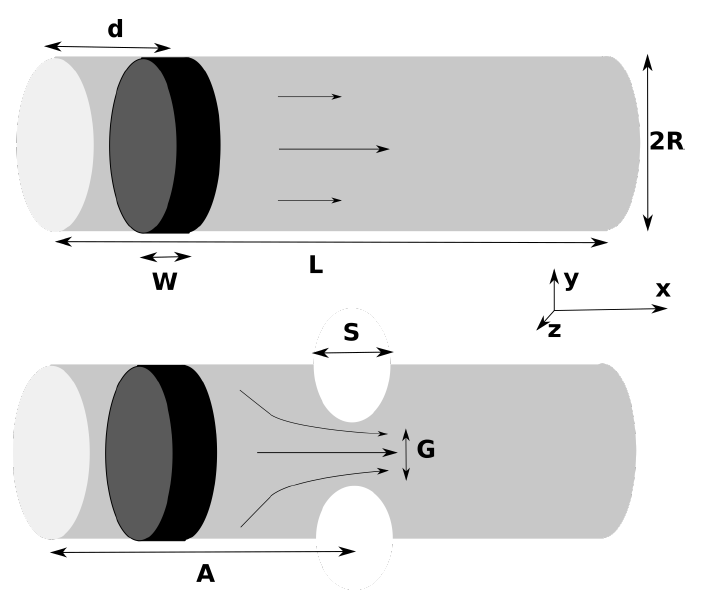
\includegraphics[width=0.40\textwidth]{artery_geometry.png}
\caption{Artery Geometry.}
\end{figure}

We used the \texttt{ShapePainter} to create the geometry, in which there are two files of particular interest:
    \begin{enumerate}
        \item \texttt{preproc1.py}: Uses a 3d canvas to create the shape and then marching cubes to generate the surface. Change the variable $Re$ to get the desired the radius and length of the channel. For $Re=10$, this script takes around 10 minutes to run.
        \item \texttt{preproc2.py}: Created \texttt{RBC.xyz} and \texttt{atom.inp} objects based on the channel. Originally for $Re=10$ it took 8 hours to finished 22\% of the job, which would need about 40 hours to finish the whole RBC implementation. Thanks to the update in the \texttt{MAGIC} backend \texttt{Fortan} code, it took less than 10 minutes to finish the RBC creation.
    \end{enumerate}
    
\begin{figure}[H]
    \centering
    \includegraphics[width=0.5\linewidth]{project2/channel.png}
    \caption{Geometry generated for Re = 10 case.}
    \label{fig:my_label}
\end{figure}

The next code we wrote is the Python script that runs the simulation on MUPHY.
Each simulation run had a file, conventionally named \tty{run2.py}, that kicks off the simulation.  
The script that ran our baseline simulation is located in 
\tty{scratchlfs/ac290r/project2/blood\_cells/BUFFY/RBC\_0\_Re10}
(We tried to follow advice given to use organized directory names.
While this is a bit long and slightly cryptic, we did at least follow a consistent scheme
this time organized everything hierarchically!)
We've included a copy of this file in project repository as well in
\tty{project2/BUFFY/RBC\_0\_Re10} for convenience in grading our submission.
\begin{figure}[h!]
    \centering
    \includegraphics[width=0.5\linewidth]{project2/directory.png}
    \includegraphics[width=0.4\linewidth]{project2/buffyfolder.png}
    \caption{Sample subdirectory in \tty{BUFFY} directory.}
    \label{fig:my_label}
\end{figure}

In summary, \tty{scratchlfs/ac290r/project2/blood\_cells/MUPHY/MAGIC} is our backend library, and in \tty{scratchlfs/ac290r/project2/blood\_cells/BUFFY/} each subdirectory represents each simulation with different RBC and Reynolds number. The basic workflow is to first create shapes in \tty{ShapePainter/}, copy the output files into their respective \tty{RBC\_X\_ReX/} folder, and submit batch scripts.



The first part of this file sets the physical parameters for the simulation,
e.g. the geometry of the cylinder and the viscosity.
The Python module \tty{MagicUniverse} is the fancifully named interface to the BUFFY simulation engine.
The script initializes simulation objects including:
\begin{itemize}
\item Universe
\item Scale
\item Mesh
\item Fluid (for blood)
\item Fluid (for drug)
\item Atom (for RBC)
\item Tracker (for diagnostics)
\end{itemize}
These are all class instances from the \tty{MagicUniverse} module.
Parameter values are set to the appropriate class instances.
We set the boundary conditions to be periodic on the $z$ axis,
and no-slip on the $x$ and $y$ axes.
The alternative configuration would have been to create inlets and outlets
at the start and end values of $z$.

We want to release the drug when the blood flow is stable, at $Re=10$ we have two relaxation time that would impact the choice of the drug release time
\begin{gather*}
    \tau_{\nu_1} = \frac{L^2}{\nu} = \frac{1000^2}{0.1} = 10^7 \\
    \tau_{\nu_2} = \frac{D^2}{\nu} = \frac{100^2}{0.1} = 10^5 \\
    \tau_{u} = \frac{L}{u} = \frac{1000}{0.01} = 10^5
\end{gather*}
Note that we choose $\tau_{\nu_2}$ with $D$ instead of $L$ because the diffisivity phenomenon is local and we do not need the whole length of the channel to expect its motion. Since $\tau_{\nu_2}$ and $\tau_{u}$ have the same order of magnitude, we choose the drug release time for $Re=10$ to be $t = 100000$.

To run this code on Odyssey (Harvard's supercomputing cluster in Western Massachusetts)
we also wrote shell scripts that were submitted to the Odyssey job manager \tty{slurm}.
The script to run the baseline simulation is called \tty{runrbc\_0.sh} and is located adjacent to \tty{run2.py}.  
The key lines in this script set the job options and load the required modules.  
Important flags include:
\begin{itemize}
\item \tty{-p shared} - run the job on the shared partition
\item \tty{--reservation=ac290r} use the reservation so we don't have to wait in the queue to get 1024 cores 
\item \tty{-t 1200} hold the job open for up 1200 minutes = 20 hours
\item \tty{-n 512} run on a total of 512 CPU cores
\item \tty{N 16} run on 16 nodes; we are therefore requesting 16 nodes with 32 cores each
\item \tty{mem=64000} request 64,000 MB = 64 GB per node; that is a lot of memory, 1024 GB = 1 TB total
\item \tty{--job-name=RBC0RE10} the descriptive job name refers to 0 red blood cells and Reynolds Number 10
\item \tty{--output=RBC0RE10.out} the directory where output is written; matches the job name
\end{itemize}

The rest of the script loads the required modules and sets environment variables.
We need modules for \tty{gcc} and \tty{openmpi}, provided by 
\tty{gcc/7.1.0-fasrc01} and \tty{openmpi/3.1.1-fasrc01} respectively.
The environment variables to set are \tty{MOEBIUS\_PATH} and \tty{PYTHONPATH}.
These allow Python to find the MAGIC modules.
In order to invoke the job as a Python 2 script with MPI, the 
line of the script that kicks off the actual job is\\
\tty{srun -n \$SLURM\_NTASKS --mpi=pmi2 python2 run2.py}

The last major batch of code we wrote performs calculations at the post-processing stage.
This is in two Python scripts \tty{vtk2np.py} and \tty{rbc.py} located in the folder \tty{project2/src}.
The MUPHY simulation generates output in the form of VTK files with the extensions .vtu and .pvtu.
These files are well suited to visualization, especially intensive visualizations like movies.
For computations and 2D plots of one time instant, we find it more convenient to use 
\tty{numpy} and \tty{matplotlib}.

We made a strategic decision to do the computationally heavy graphics rendering remotely on Odyssey
but to do the computations and 2D ploting locally on a few selected time frames.
After our baseline simulation ran, we downloaded snapshots every 100,000 frames from 100,000 to 1,000,000.
Each time step corresponds to 1 microsecond, so these frames were 100 milliseconds apart for
the first 1.0 second of the simulation.  
These files weren't too large, with a total size of about 9 GB each for the blood and drug for a total of 18 GB.
Downloading these files was a bit painful though because SFTP connections to Odyssey 
are considerably slower than data downloads from large commercial websites for whatever reason --- 
we believe that \tty{scratchlfs} might be behind this slowness.

The script \tty{vtk2np.py} converts the VTK files to numpy arrays using the library \tty{vtki}. We initially started to convert these files using the \tty{vtk} library, but we quickly realized that it was quite verbose. We later found out that the other team was discussing with the developers of \tty{vtki} to add the capacity of reading \tty{.pvtu} files directly, which was added less than 2 weeks ago! A .pvtu file is essentially a wrapper around a number of .vtu files, each with one part of a larger mesh. VTK provides various types of files, like \tty{.vti}, \tty{.vtp}, \tty{.vtu}, and so on, with their counterparts prepended with \textit{p} defining the parallel wrappers. Note that these store information as XML documents.
In our case, we ran on 512 nodes and each time step generated 512 .vtu files --- which are vtkUnstructuredGrids --- that were summarized by 1 .pvtu file.  
These outputs were generated for both blood and the drug.
The VTK files include data that is keyed both by \textit{points} and \textit{cells} on the mesh.
These are not the same! Our mesh for $Re=10$ had 7,022,647 cells and 8,578,503 points.
One important optimization is to realize that the geometric layout of the mesh does not change between frames.  
While the files contain the whole grid every time, it is only necessary to save the point and cell position data once.  
Only the density, velocity, and shear stress change over frames.

\tty{vtk2np.py} extracts and saves the following data from the VTK files as Numpy arrays:
\begin{itemize}
\item \tty{point\_pos.npy} - the (x, y, z) position of each point on the mesh
\item \tty{cell\_pos.npy} - the (x, y, z) position of each cell center of the mesh
\item \tty{cell\_vol.npy} - the volume of each cell in the mesh
\item \tty{drug\_framenum.npy} - the volume of the drug in each cell of the mesh at this frame
\item \tty{drug\_point\_framenum.npy} - the volume of the drug at each point on the mesh at this frame
\item \tty{vel\_framenum.npy} - the blood velocity at each point on the mesh at this frame
\item \tty{vel\_cell\_framenum.npy} - the blood velocity at each cell on the mesh at this frame
\item \tty{rho\_framenum.npy} - the blood density at each cell on the mesh; proportional to pressure
\end{itemize}
This program was run once locally to create numpy arrays, allowing the
next Python program to run without worrying about VTK data structures.

\tty{rbc.py} performs all the requested calculations and generates the 2D plots presented 
below that were not generated remotely using Paraview. \\
\tty{drug\_delivery} answers the headline question of how much drug is in the stenotic
region as a function of time.  
We estimated this by summing up the density of drug in the cells in the stenotic region.
We extracted the velocity of each cell and found that they were all equal to 1.
(We knew that the interior cells should have a volume of 1 because they were cubes
with side length 1, but didn't know how MUPHY and VTK handle cubes on the boundary.)
The total amount of drug present in a region $\Omega$ is $\int_{\Omega} \rho dV$
i.e. the density integrated with respect to infinitesimal volume slices.
Therefore, the discrete analog would be to sum up the density of each cell in the stenotic region multiplied by its volume.  
Since all the cell volumes are equal to 1, we omitted the multiplication from the calculation to improve performance.
We also computed the total quantity of drug in the system as a quality check, expecting it not to change.\\
\tty{plot\_speed\_contour} creates a contour plot of the speed on a cross sectional slize $z=z_{plot}$.
While we computed drug quantities using cells, we chose to plot speed using points.
The main programming challenge is generating a contour for data that doesn't cover an entire rectangular grid.
This was done by creating an augmented grid with the full square cross section containing
the circular cross section of the artery.
Grid points outside of the artery were marked with a speed of 0, which was excluded from the
range of values in the contour.\\
\tty{plot\_streamlines} plots streamlines of the velocity in the $xy$ plane
(i.e. velocity components $u$ and $v$) on a cross-sectional slice $z=z_{plot}$.
Like the speed contour, this plot uses points rather than cells.
It uses the same technique as \tty{plot\_speed} for padding the circular region
with dummy entries that don't appear on the plot.
Streamlines are plotted with a width proportional to their speed in the $xy$ plane.\\
\tty{plot\_drug\_conc} plots the concentration of the drug on a cross sectional slice $z=z_{plot}$.
This plot uses cell data.  
A mask is created using the relationship that $z$ at the center of a cell is equal to 
$z$ at the start of the cell plus $\frac{1}{2}$.  
This was preserved exactly by VTK so we could create a logical mask efficiently.
The conentration of drug at each $(x, y)$ point is then read right off the masked array.\\
\tty{plot\_drug\_profile} plots the ``profile'' of the drug along the $z$ axis for a given time.
This calculation is also based on cells.  
A mask is created for each value of $z$ as before, and the total amount of drug 
at this longitude is estimated as the sum of the drug concentration array on the mask.
An initial attempt at plotting this profile showed some obvious artifacts where 
a handful of $z$ values had ``holes'' where the dropped well below their neighbors.
We appplied a smoothing operation before plotting the profile $B(z)$ in which 
we set each $b_z$ equal to the max of itself and its two neighbors $b_{z-1}$ and $b_{z+1}$.\\
Plots of each type are displayed below in the Results section.

\newpage

\section{Parameters of the Simulation}
These are the parameter values that we set at the start of the Python script for the baseline simulation
with 0 red blood cells and a Reynold Number of 10.
\begin{itemize}
\item $\nu$ = 0.1 --- this is the kinematic viscosity
\item $\rho$ = 1 --- the blood density was set to 1 by convention
\item $\bar{u}$ = 0.01 --- this is the mean speed of the blood
\item Re = 10.0 --- the Reynolds number is dimensionless and characterizes the turbulence / regularity of the flow
\item Pe = 10.0 --- the Pectet number is dimensionless and characterizes the importance of radial to axial diffusion
\item R = $\nicefrac{Re * \nu}{2  \bar{u}}$ --- the radius is implied by Reynolds number and velocity
\item DIFFUSIVITY = $\frac{\bar{u} * R}{Pe}$ --- the dynamic viscosity applied to the drug fluid
\item C0 = 0.01 --- the baseline drug concentration away from the bolus
\item C1 = 1.0 --- the high drug concentration on the bolus at $t=0$
\item NSTEP = 1000000 --- total number of simulation steps; each step is one microsecond
\item NDIAG = 100 --- interval between diagnostics
\item NVTKFREQ = 1000 --- interval between VTK output frames
\item UNFREEZE\_TIME = 100000 --- number of time steps for the system to equilibrate before drug release
\item GROWTIME = 2000 --- number of time steps for the RBC to settle before blood flow
\end{itemize}

Given that we are dealing with a periodic system, we impose a homogeneous along the blood flow direction, the z-axis, which is also initialized in the Python scrip.t Our goal was to also run a big simulation.  
This was to be similar to the baseline, but would also include a large number of red blood cells.
These red blood cells would be simulated as rigid particles with a position and orientation.
Including the red blood cells makes the simulation more physiologically realistic,
with increasing importance the narrower a blood vessel is.
Our initial attempt was a 30\% hematocrit with otherwise identical parameters to the baseline case.  
Unfortunately multiple attempts to simulate the system with large numbers of red blood cells failed.
We will explain in detail the various failures and their causes in the section below.
Fortunately, we did complete a successful run of the baseline case without red blood cells.
We have made the best of a difficult situation by performing a complete analysis on the baseline case.

\newpage
\section{Results}

\subsection{Failed Runs on Odyssey with Red Blood Cells}
We well understand the complexities and potential difficulties of running large parallel software on clusters, and indeed our experience greatly reflected this essence. Though we fail to get our expected results from this run, we reckon the importance of documenting the distinctive errors we received in running the jobs as a good learning experience of high performance computing.

Before we launched our two simulations on the reservation, we did some test runs on smaller systems. Since the $Re=10$ with 30\% RBC has a very large system, which would take much longer time to reach the drug release time, we used the smaller systems to test the applied forces and unfreeze time of the drug. After confirming the case without RBC case worked for a smaller case, we started to test the case with RBC, which is a much bigger system. We first tried on $Re=5$ with 2\%  RBC, unfortunately it failed between $t=901$ and $t=1001$, which we suspected $Re=2$ system was too small to be parallelized, therefore we stick to the test runs on $Re=5$ and $Re=10$. However, both case also failed between $t=901$ and $t=1001$ with the same memory leak issue. Luckily this memory leak was fixed on the first day of scheduled run.
\begin{figure}[H]
    \centering
    \includegraphics[width=\textwidth]{doublefree.png}
    \caption{Screenshot of a portion of error message due to memory leak.}
    \label{fig:memory_leak}
\end{figure}

    
Having tested on smaller systems, our actual runs still turned into a log of struggles on Odyssey. Various exit codes emerged during the process, and some errors were very unexpected: Having changed nothing to the code, the program suddenly reported Segmentation Fault and MPI Communication error. Even though the popular belief says that ``insanity is doing the same thing over and over again and expecting different results'', submitting the same job multiple times ended up fixing the error (one success for every ten failed submissions). The diagnosis is clear: we are definitely insane. On a more serious note, it seems like some part of the program (or Odyssey) displays some Byzantine behaviour.

Now, we will go through our run history. For simplicity, \textbf{Re=10, RBC=0\%} represents the simulation of 0\% red blood cells at Reynolds number =10.

\textbf{Re=10, RBC=0\%:}
The test runs we had were run on either $64$ or $128$ cores, when we used the full 1024 cores reservation, it gave continuous segmentation fault when we outputted the first VTK file at $t=1000$. Then, we tried to specify the partition to be $7$, which is partitioning in parallelepipeds for a generic number of MPI tasks. However, this still did not run. We ran on $512$ cores with \texttt{m.setPartitionAlongXYZ(2,2,128)}, and the job took around 8 hours to finish.

\textbf{Re=10, RBC=30\%:}
Our initial attempts to run the case with RBC were not very successful, and we waited until the memory leak was fixed to run the actual 30\% job. It ran for around 10 hours and failed with ExitCode 1. It failed at the exact time (t=3000) when RBC was starting to move. The emitted signal suggested that the equilibrium was not sufficiently long and the cells collided wildly among themselves. Having read the error log, our instructor suggested this case seemed to require a long equilibrium, which defeats the purpose of the project. Therefore, we focused our RBC simulation on smaller systems.

\textbf{Re=10, RBC=5,10\%:}
When we switched to simulate on smaller systems, the program managed to go beyond the unfreeze blood flow time ($t=1.5\times2000=3000$). However, it failed around around $t=7001$, which might be caused by releasing the RBC too abruptly. We modified the code to add one more if statement to have a more gentle blood unfreeze process. However, the adjusted program ran for more than 2 hours and failed at $t=5000$ when RBC was imposed to a slightly bigger force, therefore the RBC releasing process was still too abrupt.

\begin{figure}[H]
    \centering
    \includegraphics[width=0.4\linewidth]{project2/blood_old.png}
    \includegraphics[width=0.4\linewidth]{project2/blood_new.png}
    \caption{Left: Original unfreeze blood routine. Right: Updated gentle unfreeze routine.}
    \label{fig:my_label}
\end{figure}


\textbf{Re=5, RBC=5\%}
Due to time limit we decided to work on the smallest system possible for this project. However, for some reason we fail to understand, we consistently received segmentation faults when we launched the program. The error log pointed to the fact that the segmentation fault occurred in the module load part, where we never changed since the module loading worked fine for previous runs. In addition to the segmentation fault (Exit Code 139), we also received over a dozen of Exit Code 137, which pointed to MPI communication error (InfiniBand error or failure to find nodes). Though we were unable to pin down the actual causes of both errors, we discovered that if we submitted the job multiple times, there would be one time that went through (around one in every ten submissions). The most eccentric pattern was that before we successfully ran a job, we would get Exit Code 137 and Exit Code 139 in sequence.

Our final strategy was to submit job continuously until Odyssey accepted it. There were four jobs submitted successfully, and all of them ran for a while and failed. The objective run time is 60000. The error logs were suggesting possible memory issue which we failed to trace back.

\begin{table}[H]
\centering
\begin{tabular}{|c|c|c|}
\hline
\textbf{Job Name} & \textbf{Time Steps} & \textbf{Error}                     \\ \hline
RBC5RE5           & 10001             & malloc(): memory corruption        \\ \hline
RBC5RE5           & 17201          & free(): invalid next size (normal) \\ \hline
RBC5RE5           & 21501          & corrupted double-linked list       \\ \hline
RBC5RE5           & 21501             & corrupted double-linked list       \\ \hline
\end{tabular}
\caption{Error message and elapsed time steps for Re=5, RBC=5\%}
\end{table}

In conclusion, we notice two possible sources of errors. When we first launch the job, there are chances that the cluster would emit segmentation fault on unexpected commands. And when we successfully launch the job, the software may experience a memory issue as the simulation moves further. 

\begin{figure}[H]
    \centering
    \includegraphics[width=\linewidth]{project2/exitcode139.png}
    \caption{Screenshot of a portion of error message due of module load segmentation fault.}
    \label{fig:my_label}
\end{figure}
\begin{figure}[H]
    \centering
    \includegraphics[width=\linewidth]{project2/exitcode137.png}
    \caption{Screenshot of a portion of error message due of MPI communication error.}
    \label{fig:my_label}
\end{figure}

This project had a very tight schedule due to a combination of the timing of the semester and the limited availability of computational resources. We worked diligently to achieve a successful simulation run with red blood cells, but unfortunately all of our efforts ended in failure. If we had more time and computational resources, we are optimistic that we could achieve a simulation along the lines that we attempted. We detail these failures in the table below. As a quick scan through this table suggests, we experienced a diverse range of problems, including software problems (bugs in the code base); incorrect parameter values
that needed to be adjusted; and hardware failures. Based on our job history and SLURM notifications, we listed the errors, run time and possible diagnostics that we encountered during the failed runs for RBC. 
\begin{table}[H]
\centering
\begin{tabular}{|c|c|c|c|c|}
\hline
\textbf{Job Name} & \textbf{Run Time} & \textbf{Exit Code} & \multicolumn{1}{l|}{\textbf{Count}} & \textbf{Diagnostic}                                                                     \\ \hline
RBC30RE10         &                   &                    & 2                                   & MPI communications error.                                                               \\ \hline
RBC30RE10         & 10:30:32          & 1                  & 1                                   & Equilibration was not sufficiently long. \\ \hline
RBC30RE10         & 01:33:09          & 0                  & 1                                   & Node fail.     \\ \hline                                                                         
RBC10RE10         & 03:49:42          & 1                  & 1                                   & Segmentation fault (Address not mapped).   \\ \hline
RBC10RE10         &                   & 137                & 2                                   & Segmentation fault (Address not mapped).                                                \\ \hline
RBC10RE10          & 01:34:41          & 137                & 2                                   & Releasing the cells is too abrupt.                                                      \\ \hline
RBC5RE10          & 02:56:34          & 1                  & 2                                   & Releasing the cells is too abrupt.                                                      \\ \hline
RBC5RE5           &                   & 137                & 18                                  & (MPI) InfiniBand retry count exceeded.                 \\ \hline
RBC5RE5           &                   & 139                & 29                                  & Segmentation fault when loading modules.                                                \\ \hline
RBC5RE5           &  02:08:38        & 1                & 1                                  & Adjusted cell release is still abrupt.                                                \\ \hline
RBC5RE5           &  01:56:47        &                 & 4                                  & Corrupted double-linked list.                                              \\ \hline
RBC0RE10           &  02:06:40        &                 & 1                                  & Segmentation fault when loading modules.                                              \\ \hline
\end{tabular}
\caption{History of failed RBC simulations on Odyssey.}
\end{table}

Fortunately we did achieve one successful run of our baseline case without red blood cells. In the section below, we outline our results in that baseline case. Overall, though our communication with Odyssey on RBC simulation did not go as smoothly as we expected, we still value this project and take it as an excellent learning experience with high performance computing. Here are our key takeaways:
\begin{enumerate}
    \item Before launch the full-size simulation, it is always good to prepare some smaller-scale test runs. With those test runs we are able to pin down some parameter tuning issue or some potential parallel computing issue. Also test runs allow us to estimate the total run time for the actual simulation.
    \item \tty{/n/scratchlfs} may be very unresponsive, and data transfer from Odyssey is very time consuming and slow. Therefore, for post-processing we need to be aware of the size of files and the time of downloading, and decide the best approach to either work remotely on Odyssey or locally.
    \item Some errors are expected, therefore we need to be calm and spot the error, or test on smaller scales, or resubmitting the jobs till Odyssey accepts it. However, it seems obvious that at least some part of the whole pipeline is not resilient enough to faults, which are meant to occur in highly distributed systems like this one.
\end{enumerate}


\subsection{Drug Delivery Over Time}
As described in greater detail in the Description of Code, we computed the quantity of drug
in the stenotic region and the whole system by summing the density over cells.
This was a simple sum of the density because each cell has a volume of 1.0.
In general, we would need to sum over concentration times cell volume.
We started by computing the total amount of drug simulated to be in the system,
because it should remain constant after the simulation starts.
Our first attempt at this calculation incorrectly used points rather cells, and we noticed
 a marked increase in drug over the first 1.0 second, greater then 10\%.
This was an indication something was wrong and we realized we needed to use cells.
Here is the plot of drug volume in the system.  
The axis is scaled to start at zero so our eyes can read off the magnitude of the fluctuation
in this ostensibly invariant quantity.  
The simulation has the total quantity increasing by 3.59\%.
\begin{figure}[H]
\centering
%\hspace*{-0.25in}
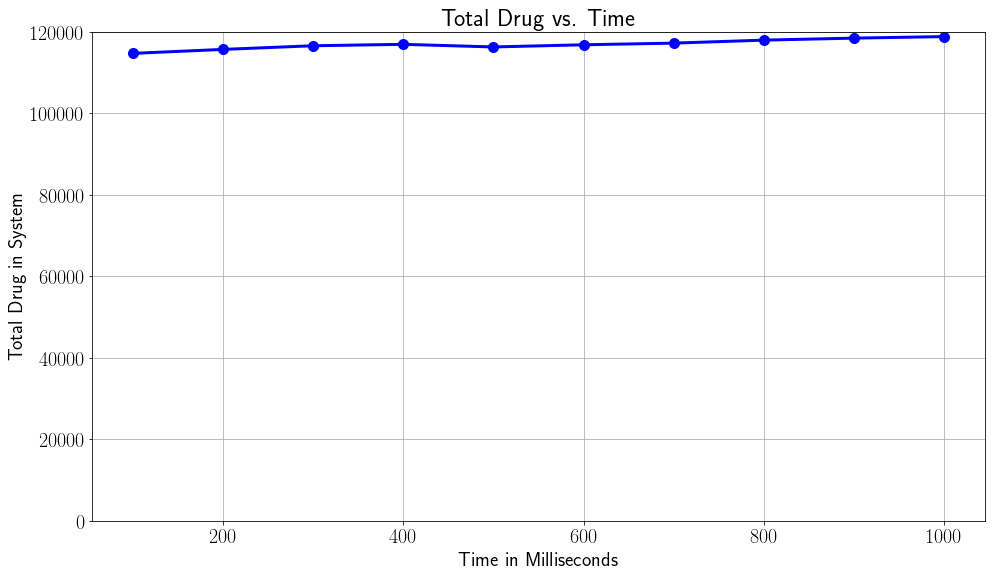
\includegraphics[width=\linewidth,height=9cm]{drug_tot.png}
\caption{Total Drug Quantity in the System Over Time}
\end{figure}

Here is the requested plot showing the quantity of drug in the stenotic region.
Because the absolute units in this problem are somewhat arbitrary,
we are presenting the amount of drug in the system as a fraction of the total.
We show the fraction in the stenotic region over time as the blue series.
We compare this to a flat line in red, which is the fraction of the total volume
occupied by the stenotic region.  
This was computed by counting the cells in the stenotic region using the same
mask we used for the drug quantity.  
(The sum of volume is a simple cell count since each cell has volume 1.0).
When the system reaches equilibrium, we would expect the drug to be completely
diffused and at a uniform concentration.  
In that case, the fraction of drug in the stenotic region would be equal to the volume fraction.  
By comparing these two quantities, we can develop an intuition as to how much 
the drug has been delivered vs. its equilibrium.
\begin{figure}[H]
\centering
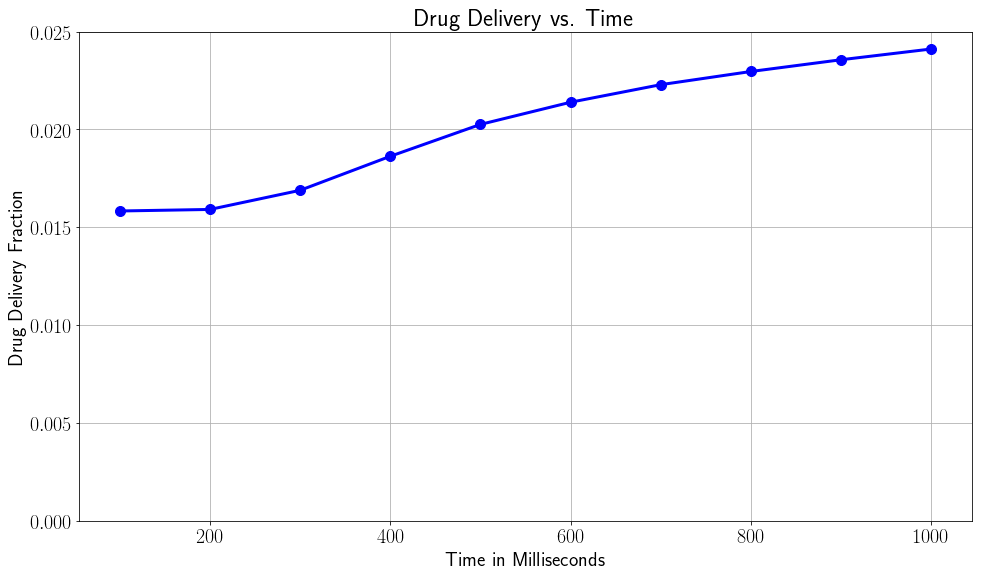
\includegraphics[width=\linewidth,height=9cm]{drug_frac.png}
\caption{Relative Drug Delivery to Stenotic Region Over Time}
\end{figure}
We can see that by the end of the first second, the drug delivery
is approaching its equilibrium level, showing that it disperses quite rapidly.

\subsection{Velocity Field - Contours of Speed and Streamlines}
Here are two plots showing the contours of flow speed at time t=800 milliseconds, 
when the flow is fairly well established.  
We plot cross sections at two locations: 
the center of the stenosis, $z=500$,
and to the right of the stenosis at $z=800$.
At the center of the stenosis, we can see that the flow is fastest in the center, and slowest close to the walls, as we would expect.
The difference in speed is less pronounced but still present away from the stenosis.
There is also an interesting effect where the speed is greatest not at the center, but to one side.
This is not a permanent feature of the flow; the ``hot spot'' moves around.

\begin{figure}[H]
\centering
\hspace*{-0.25in}
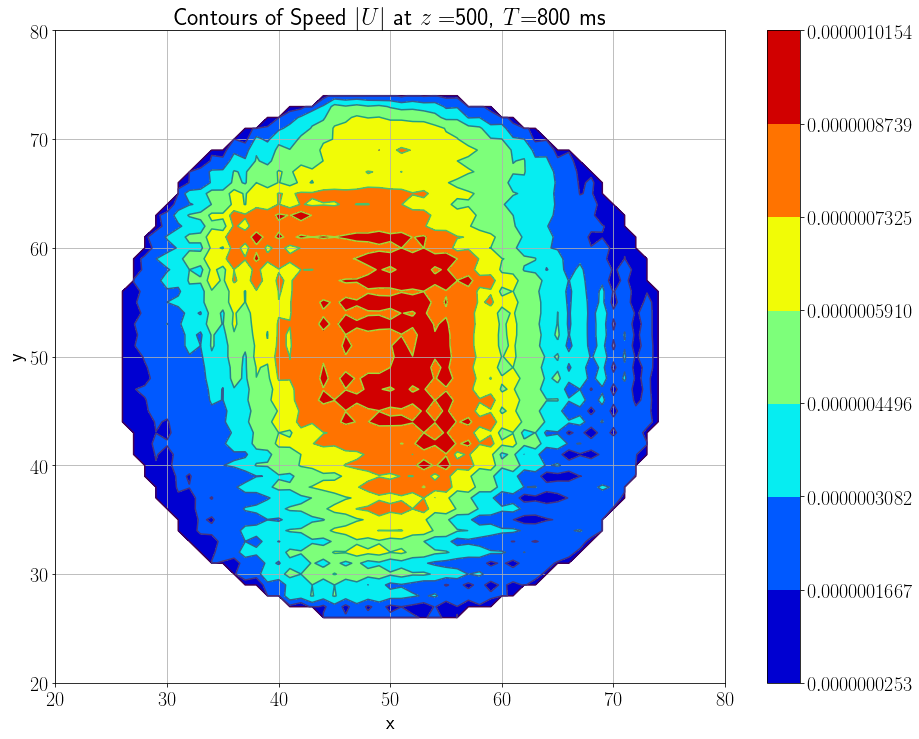
\includegraphics[width=0.75\textwidth]{contour_speed/contour_speed_z_500_t_800.png}
\hspace*{-0.25in}
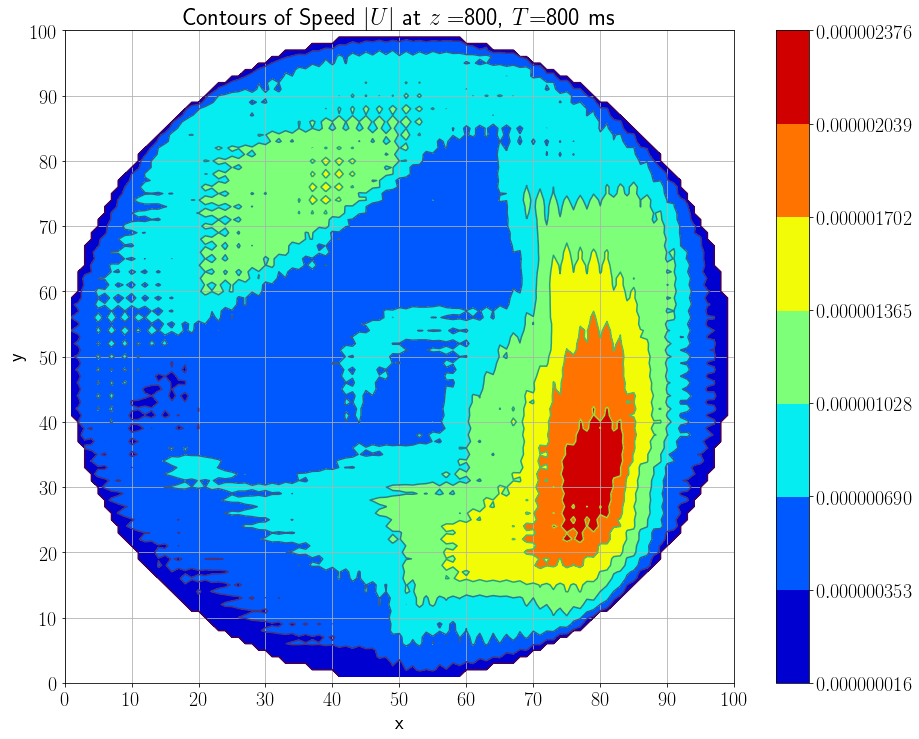
\includegraphics[width=0.75\textwidth]{contour_speed/contour_speed_z_800_t_800.png}
\caption{Contours of Speed at time t=800 ms; at two locations, center and right of stenosis}
\end{figure}

Here are two analogous plots for the same two time instants and $z$ cross sections showing
streamlines in the $XY$ plane instead.
In looking at these plots, we are becoming suspicious that there may have been a 
conceptual error in the boundary conditions.  
Dr. Melchionna suggested that we set the periodicity flag to `111' indicating that all three
components $x$, $y$ and $z$ have periodic boundaries.
We had initially planned on setting this parameter of `001' indicating that the $z$ axis
was periodic, but $x$ and $y$ were not.

In looking at the last streamline plot above, it seems as if a strong flow has developed
in the XY plane that is wrapping around from the southeast corner to the northwest corner.
We are writing this remark too late in the development process 
to re-run our simulation and post-processing pipeline.  
As scientists we prefer to be honest and express some reservations about one element of this
computation than to try to sweep difficulties under the rug.
For the purposes of a course project under these time constraints, we believe this is a 
solid effort that meets the requested requirements.  
If this were a paper to be submitted to peer review or an analysis that would be used
in treating patients, we would need to do additional work to get a definitive answer about
whether the periodic boundary conditions on the $x$ and $y$ axes were incorrect.

\begin{figure}[H]
\centering
\hspace*{-0.25in}
\vspace*{-0.50in}
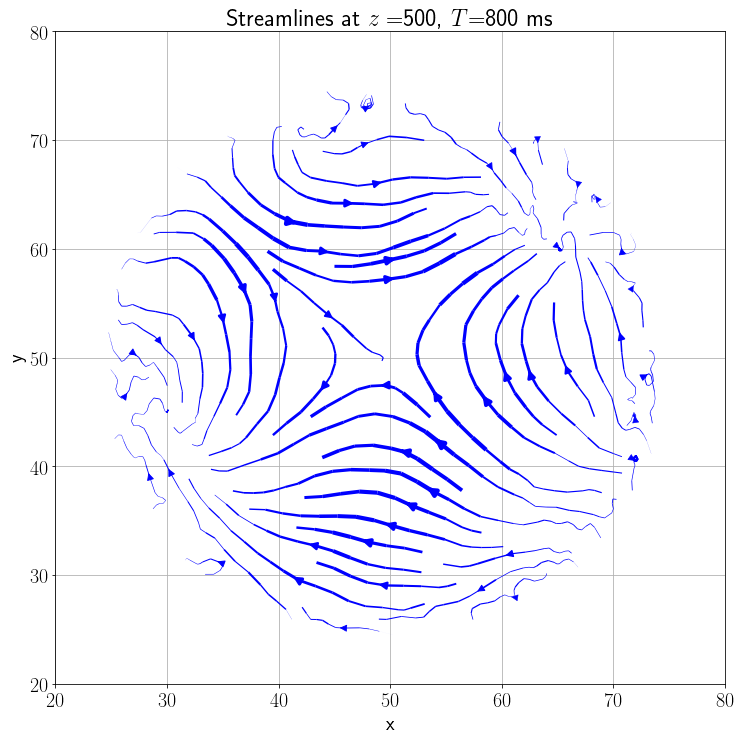
\includegraphics[width=0.75\textwidth]{streamlines/streamlines_z_500_t_800.png}
\end{figure}

\begin{figure}[H]
\centering
\hspace*{-0.25in}
\vspace*{-0.50in}
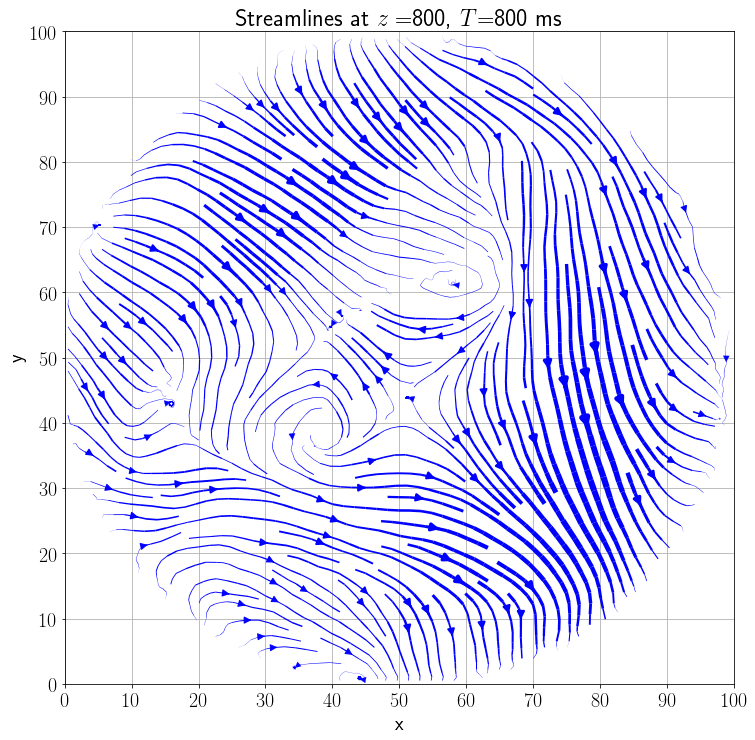
\includegraphics[width=0.75\textwidth]{streamlines/streamlines_z_800_t_800.png}
\caption{Streamlines at time t=800 ms; at two locations, center and right of stenosis}
\end{figure}

\subsection{Drug Concentration - Contours}
Here are two contour plots for the concentration of the drug at the center of the stenosis
at $z=500$.  They are run at times of 200 and 800 milliseconds.
The scale on these charts is tricky.  
There is only a very small variation in concentration between the lowest and highest end of the scales.  
Still the visual pattern is clear, and we can see that the drug concentration is highest in the
center and lower on the edges.
\begin{figure}[H]
\centering
\hspace*{-0.25in}
\vspace*{-0.50in}
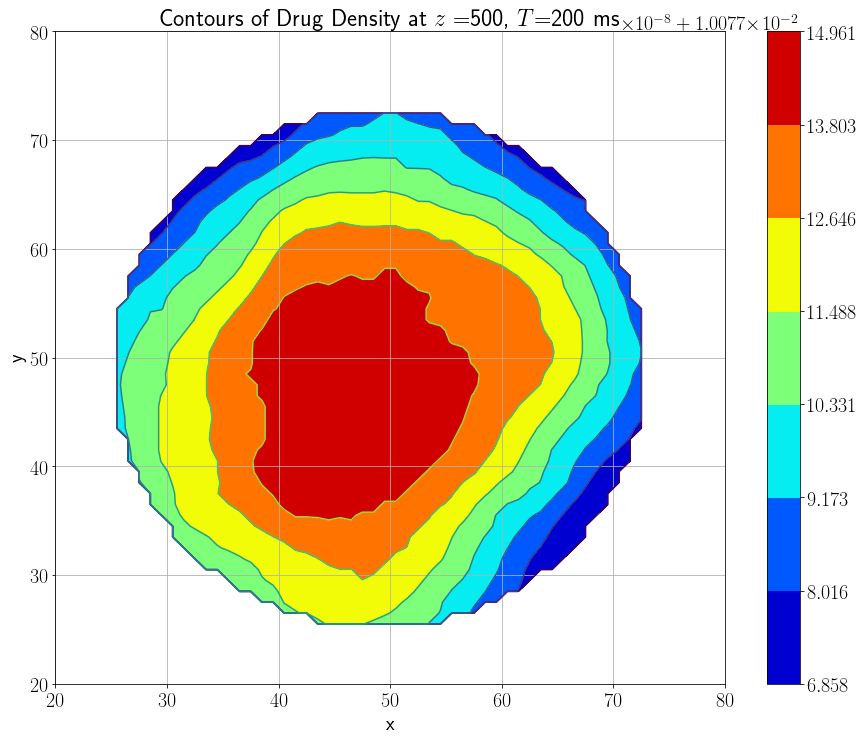
\includegraphics[width=0.75\textwidth]{contour_drug/contour_drug_z_500_t_200.png}
\end{figure}
\begin{figure}[H]
\centering
\hspace*{-0.25in}
\vspace*{-0.50in}
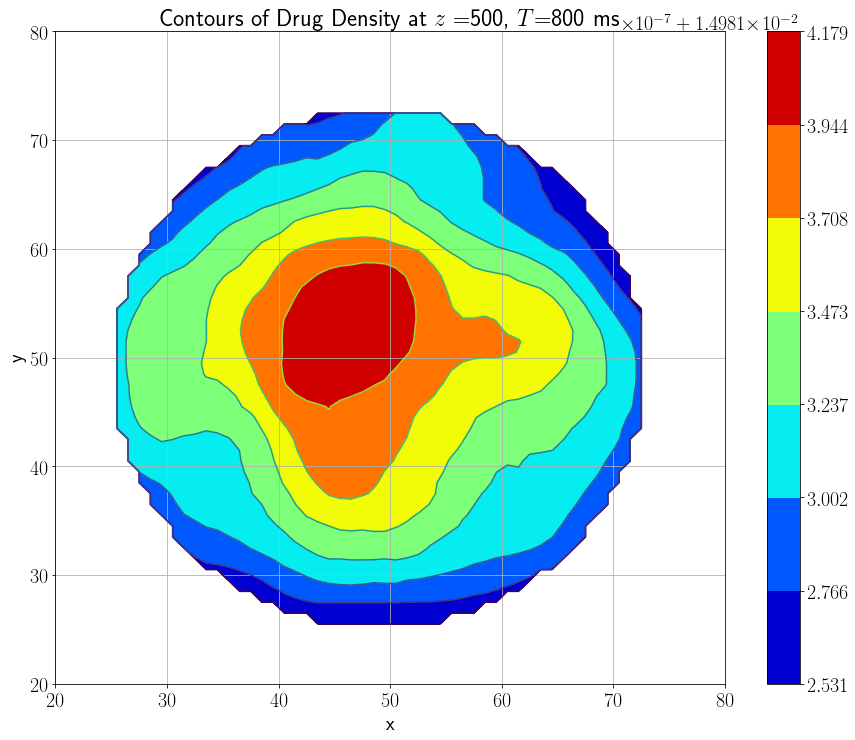
\includegraphics[width=0.75\textwidth]{contour_drug/contour_drug_z_500_t_800.png}
\caption{Drug concentration at center of stenosis at two times, 200 and 800 ms}
\end{figure}

\subsection{Longitudinal Drug Profile vs. Time}
We would like to reiterate that we needed to apply a small degree of smoothing
to generate interpretable plots for the drug profile.  
We computed the concentration as a function of $z$ and $t$ using the finest resolution
possible, $z=1$.  Mostly the results were good, with just a few artifacts.
We applied a simple filter with a width of $z=1$ to get a picture for what is really happening
in the system.  
All the plots below are scaled with the y-axis starting at zero.  
This allows us to compare profiles at different times and develop an intuition
about how the bolus migrates left to right and diffuses outward over time.
Without a common scaling, all the charts look very similar, and it is
much harder to understand the interplay between advection and diffusion.
We plot the profile at times of 200, 300, 400, 600, 800 and 1000 milliseconds.
The profile at 100 shows a spike with the density at 1.0 in the bolus and 0.01 elsewhere.
			By 100 milliseconds it has diffused and looks like a normal distribution.
			Because of the periodic boundary, the left tail of the distribution wraps around
			to the right side of the plot.  
			Over the succeeding time steps we can see the peak widening out and
			gradually drifting to the right with the advection.
			By the time we reach 1.0 seconds the profile has leveled out substantially,
			though we can still see that concentration in the stenotic region is lower.

\begin{figure}[H]
\centering
\hspace*{-0.25in}
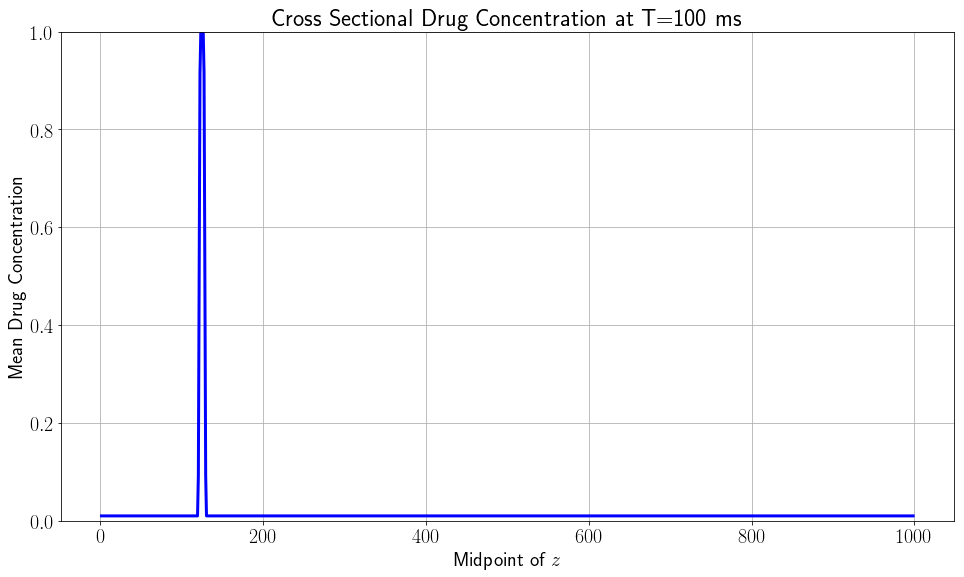
\includegraphics[width=0.50\textwidth]{drug_profile/drug_profile_t_100.png}
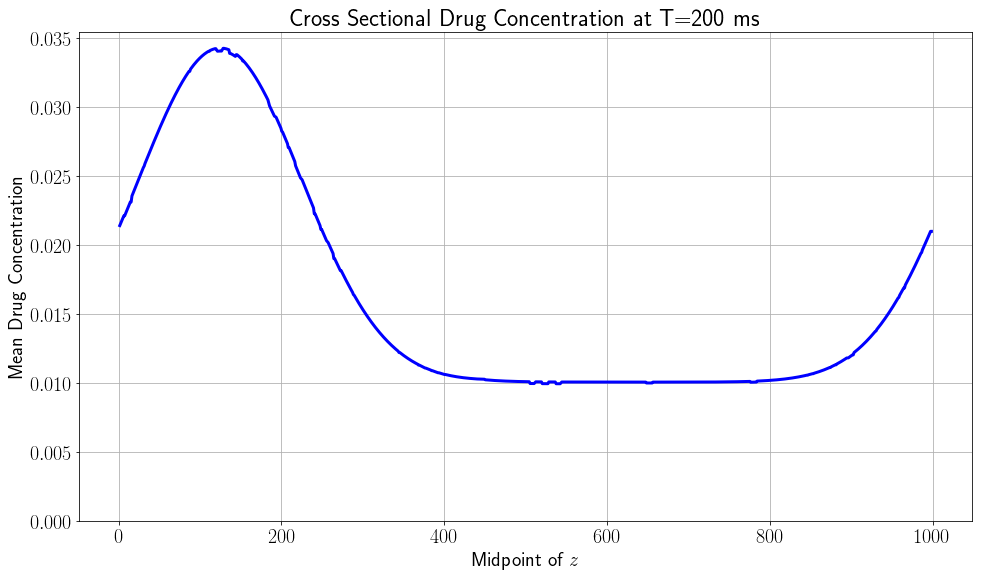
\includegraphics[width=0.50\textwidth]{drug_profile/drug_profile_t_200.png}\\[0.25in]
\hspace*{-0.25in}
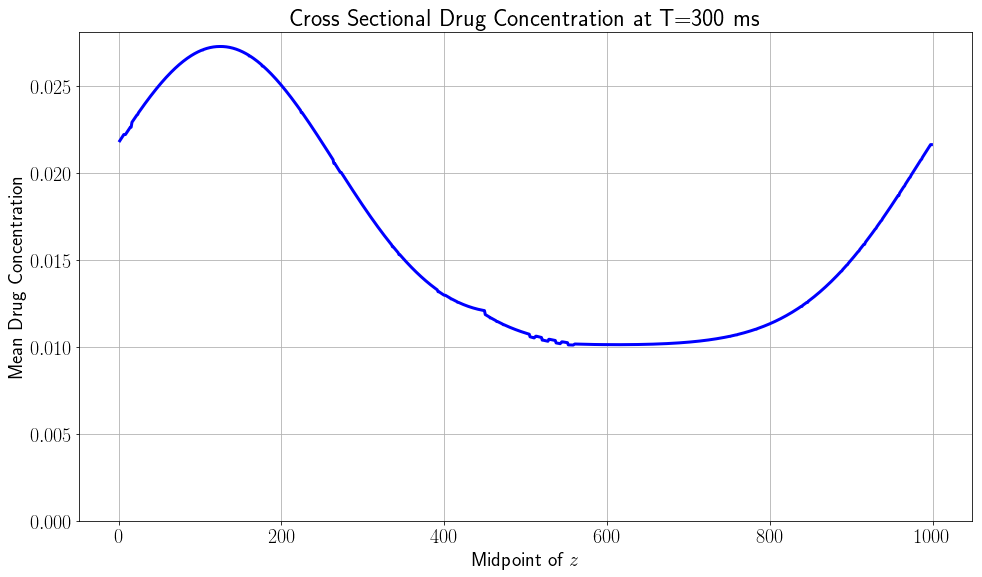
\includegraphics[width=0.50\textwidth]{drug_profile/drug_profile_t_300.png}
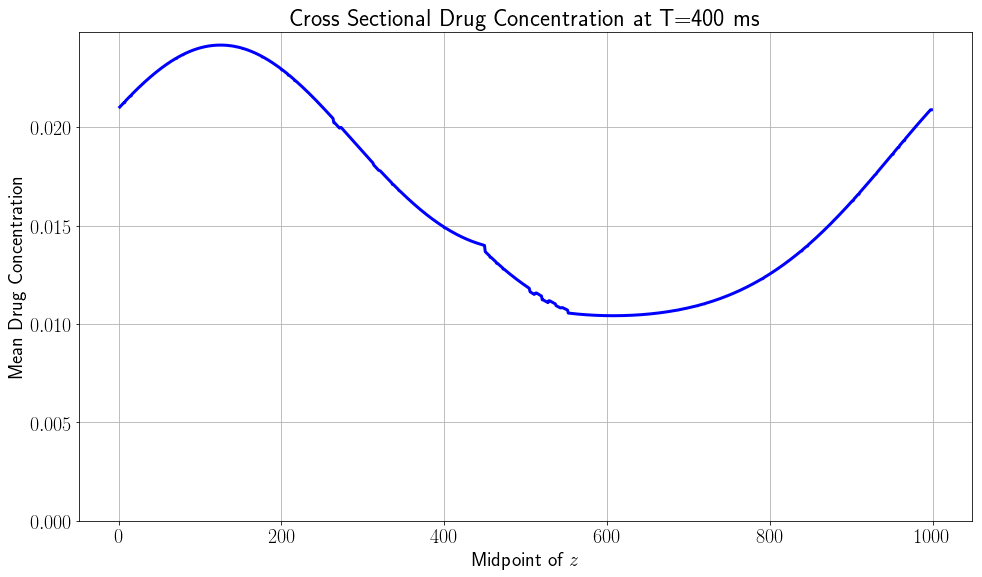
\includegraphics[width=0.50\textwidth]{drug_profile/drug_profile_t_400.png}\\[0.25in]
\hspace*{-0.25in}
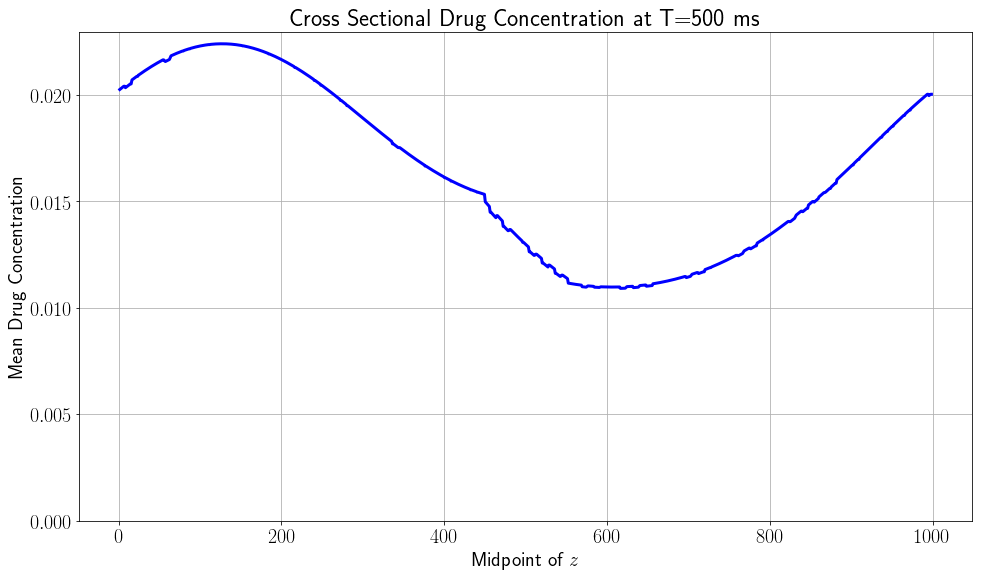
\includegraphics[width=0.50\textwidth]{drug_profile/drug_profile_t_500.png}
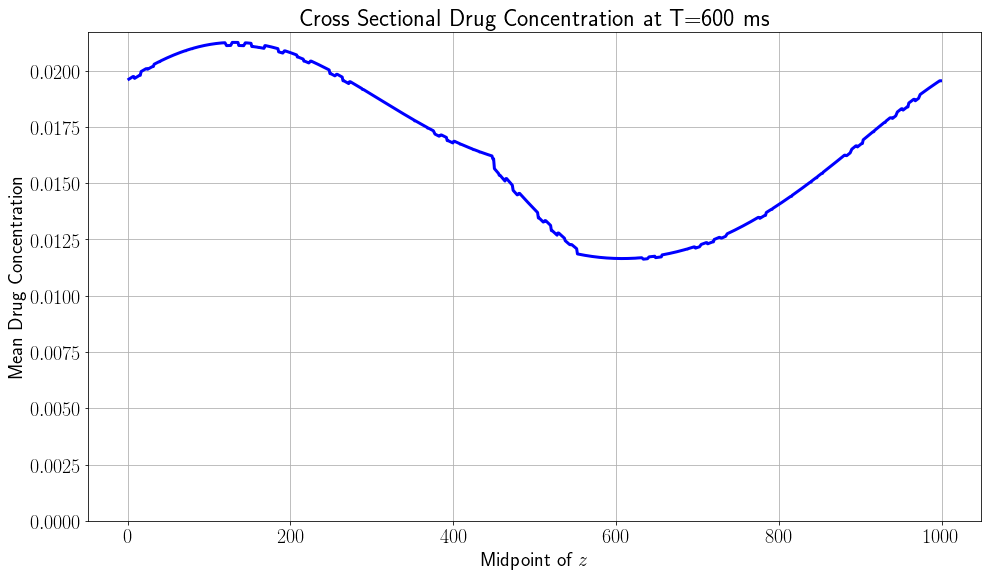
\includegraphics[width=0.50\textwidth]{drug_profile/drug_profile_t_600.png}\\[0.25in]
\hspace*{-0.25in}
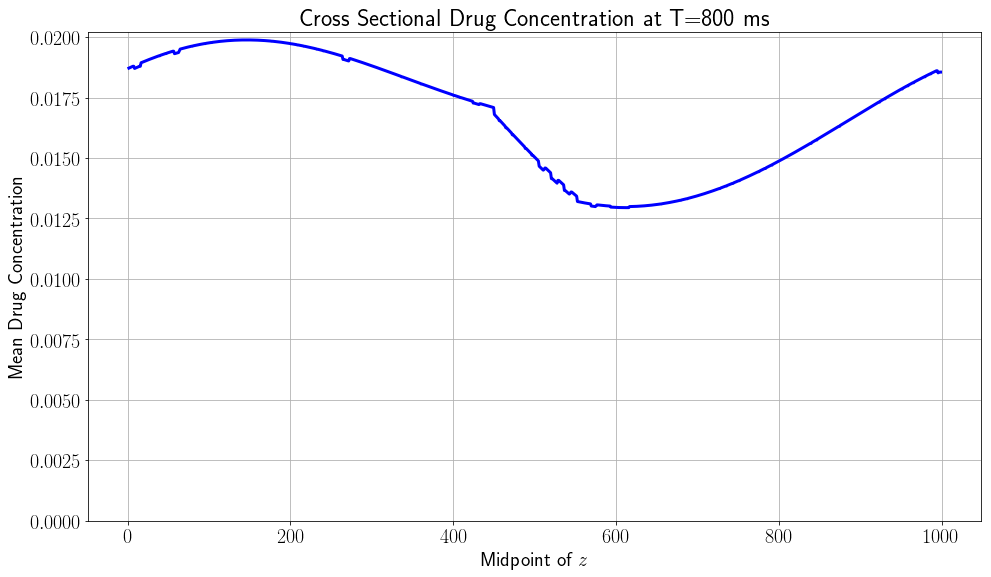
\includegraphics[width=0.50\textwidth]{drug_profile/drug_profile_t_800.png}
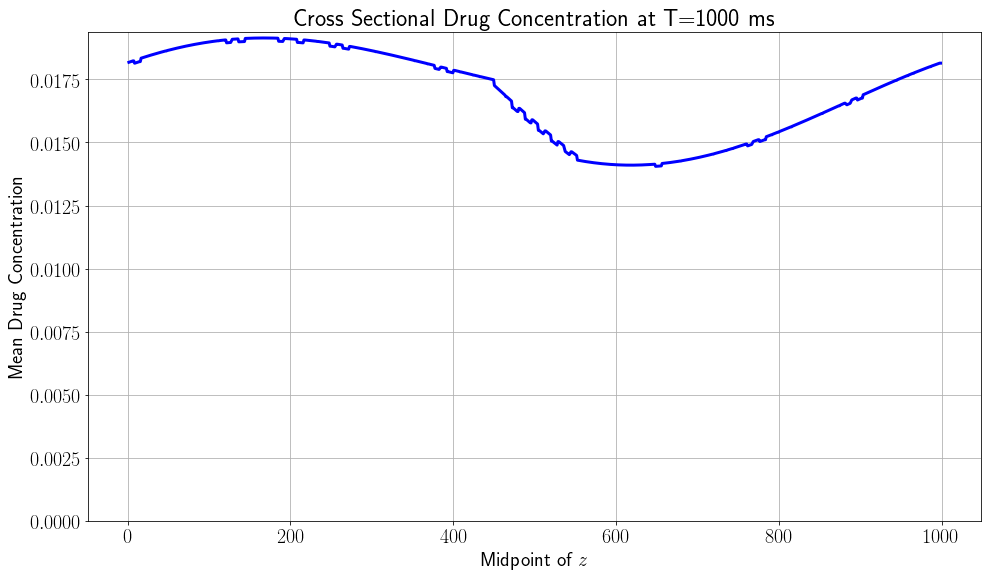
\includegraphics[width=0.50\textwidth]{drug_profile/drug_profile_t_1000.png}
% \caption{Longitudinal drug profile at times of 100, 200, 300, 400, 500, 600, 800 and 1000 ms}
\end{figure}

\subsection{Schlieren and Movies}
Like in the first module, we play around with the color palettes and created some Schlieren images. We also managed to create two movies, one details the time frames when the bolus starts to move, and the other demonstrates its long term diffusion in the blood flow. Both movies are included in the repo.

We generated the said videos using Paraview on Odyssey's virtual desktop with 8 CPU cores and 16GB of memory --- which are the max specs available. Our experience of running Paraview remotely was that it was extremely slow; once we load the desired \tty{.pvtu} files, the application reacts to interactions with a substantial delay (20-30s). You can imagine how difficult it may be to effectively drag the surface around properly with no instantaneous visual feedback. We believe that the lack of GPU acceleration (and indirectly, useful toolkits like OpenGL) on the virtual desktop is a very probable culprit; hence, we decided to submit a ticket to the Odyssey team describing this problem, and suggested that enabling GPUs when launching virtual desktop instances might be a fix --- and would be a great feature anyway. 

\begin{figure}[H]
    \centering
    \includegraphics[width=\linewidth]{project2/schlieren.png}
    \caption{Schlieren images at Z = 457, T = 50000, 70000, 80000 for Re = 5, RBC = 0\% with different color palette choices.}
    \label{fig:my_label}
\end{figure}

\newpage
\section{Conclusions and Future Work}

\subsection{Things we Learned About This Hemodynamic System and Future Work}
			In our baseline simulation, we found that a system with these physical
			parameters will get fairly close to equilibrium concentrations within a time horizon of 1.0 second.  
			If these parameters are a reasonably accurate approximation to the hemodynamics of a large
			artery receiving treatment via a bolus, the high level conclusion is that the specific geometry
			and flows are probably not that important.  
			The drug molecules are going to diffuse into the stenotic region, and the concentration will
			be near equilibrium levels by the patient's first heartbeat.
			The main conclusion from the base case may be that if we want to make useful predictions
			of drug delivery, we have to use a more realistic model of a human circulatory system
			with a more complete geometry of the arteries and veins.
			
			In light of our difficulties with the RBC simulation, and the relative lack of importance
			in larger arterial systems, the most fruitful direction for future work in this specific problem
			area would probably be for a larger, more physiologically accurate mapping of the circulatory system.  
			Computationally, the optimal direction would most likely be to shift from CPU to GPU simulations.
			
	%% bibliography		
	At this point we must address the elephant in the room: 
			all of our simulations including red blood cells ended in failure.
			Clearly, these failed simulations didn't tell us anything about the dynamics of this system.
			They did teach us about Extreme Computing.
			
			\subsection{Things We Learned About Extreme Computing}
			At the risk of a \textit{clich\'e}, the first conclusion is that Extreme Computing is ... hard.
			This is the second module, and the second time we experienced major failures on 
			our most ambitious computing job and needed to analyze a smaller job as a fallback plan.
			While running the computational jobs, we learned some common-sense principles that
			were also suggested by our instructors.  
			
			It is advisable to run smaller test cases before launching a full scale simulation.
			Some errors may manifest themselves at the smaller scale, 
			and it is less expensive in both time and computing resources to troubleshoot them
			on a smaller experimental run.
			A second lesson learned was less obvious to us.  
			Some errors have a non-deterministic (i.e. random) aspect to them,
			and submitting the same job repeatedly may help.
			This is quite different from our experience running regular-sized programs on a single
			PC, which almost always behave the same way.
			Albert Einstein is said to have quipped that the definition of insanity is doing the same thing 
			over and over again and expecting different results.
			A corollary may be that only insane people should try Extreme Computing.
			
			As we reach the end of the course, we will close with some more 
			philosophical comments about Extreme Computing.
			People are more likely to say they do something at the limits than to actually do it.
			Talk is cheap.  What does it mean to do any endeavor in the extreme?
			The sine qua non is the risk of failure.
			
			In honor of Simone's past work with the Ferrari F1 racing team, we can make this point by analogy.  
			What is the difference between driving a car and racing a car?
			When we drive, we expect to get from point A to point B, with a preference to go faster, but we are NOT willing to crash.
			When we watch a professional race car driver on TV, we expect them to go insanely fast, and accept that sometimes 
			they WILL crash (we don't accept that they will get injured anymore).
			This weekend at the Azerbaijan Gran Prix, the young star on the Ferrari Team Charles Leclerc 
			posted the best time in the last practice session, 
			then proceeded to put his multi-million euro SF90 race car into the wall. \\
			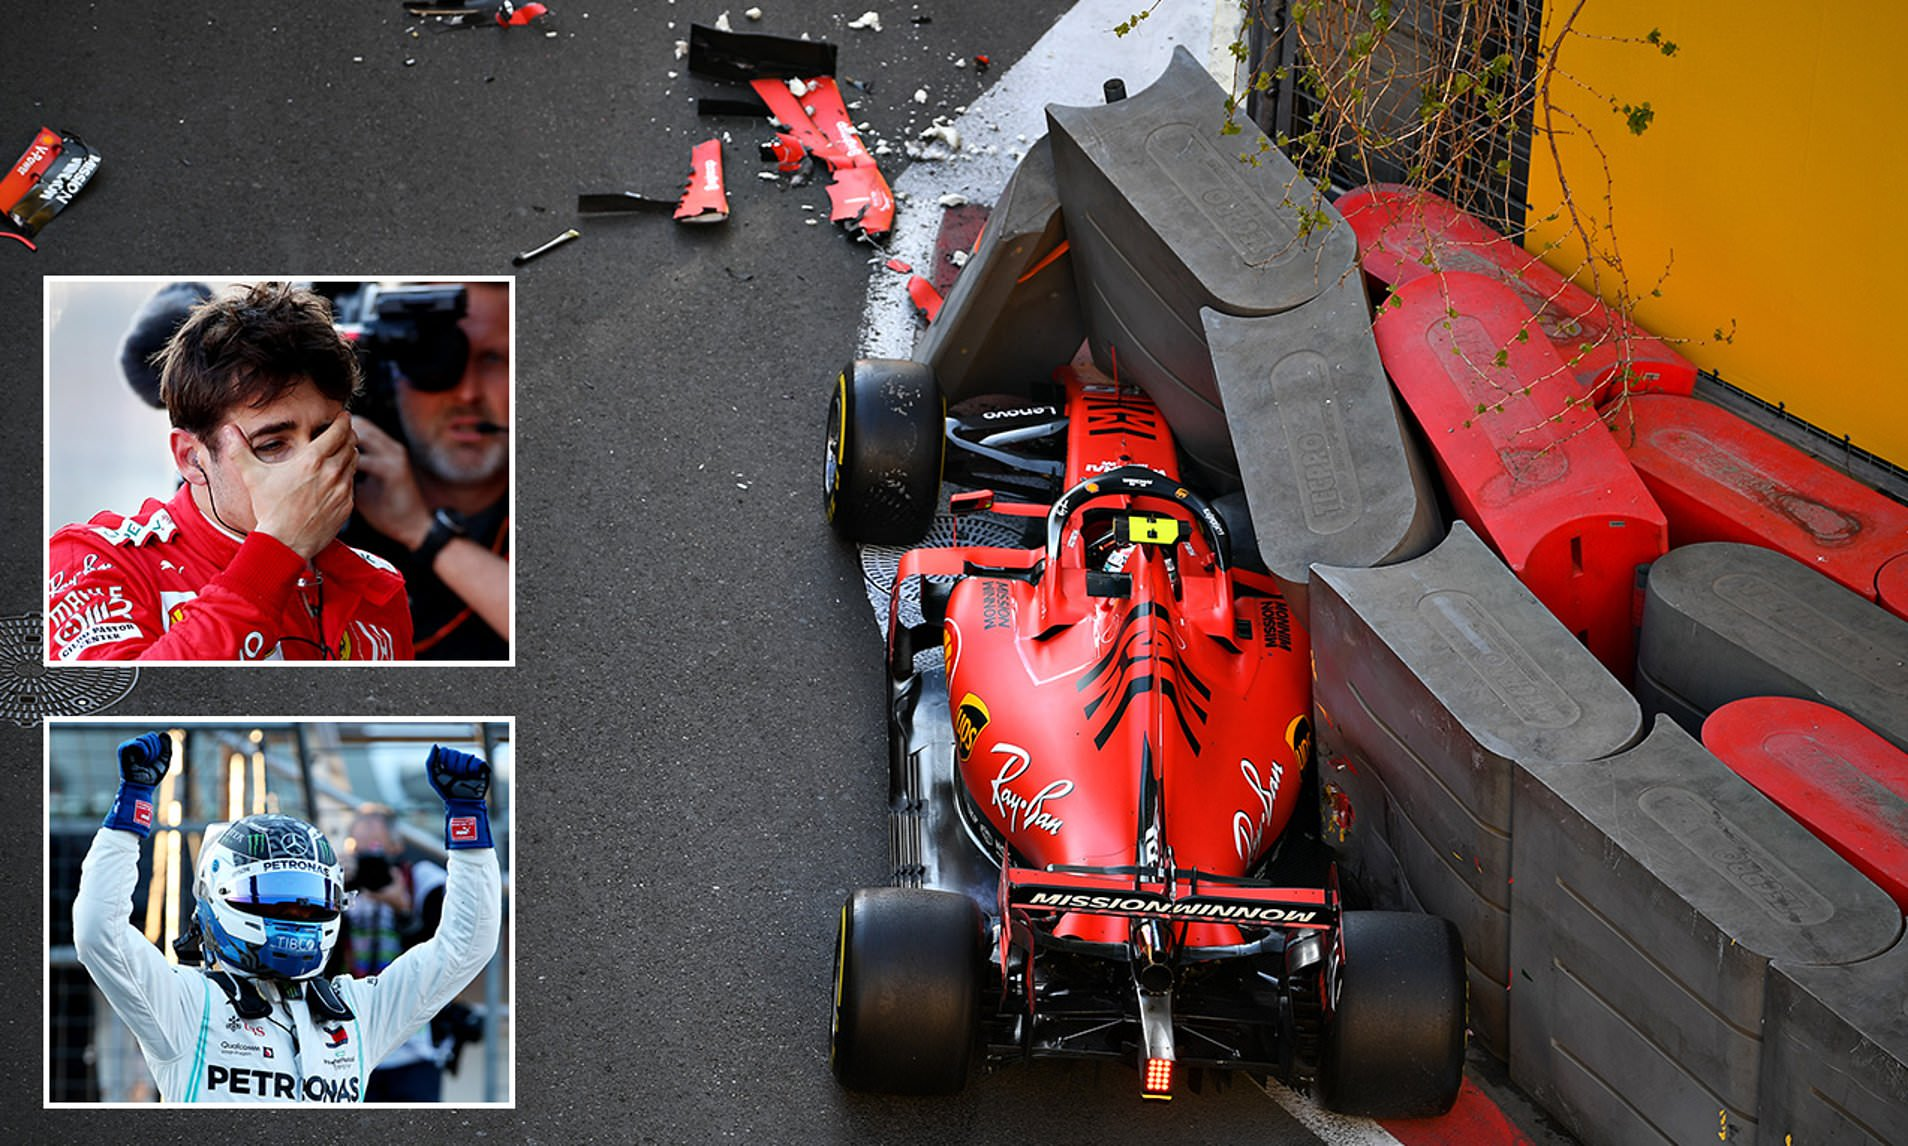
\includegraphics[width=1.00\textwidth]{pictures/charles_leclerc_crash.jpg}\\
			After the crash, Leclerc said ``I am so stupid'' on the team radio twice.
			But is he stupid? Of course not!  
			Otherwise he wouldn't be getting paid millions of euros a year to race cars
			by the most iconic team in the sport.
			In order to achieve a lap time fast enough for a shot at pole position, 
			Leclerc needed to take risks and take the preceding corner very close to the wall.
			He was the second driver of the day to crash in almost the exact same spot.
			Here is a more hopeful image.  
			It shows Leclerc being congratulated by Lewis Hamilton after his third place finish in Bahrain.\\
			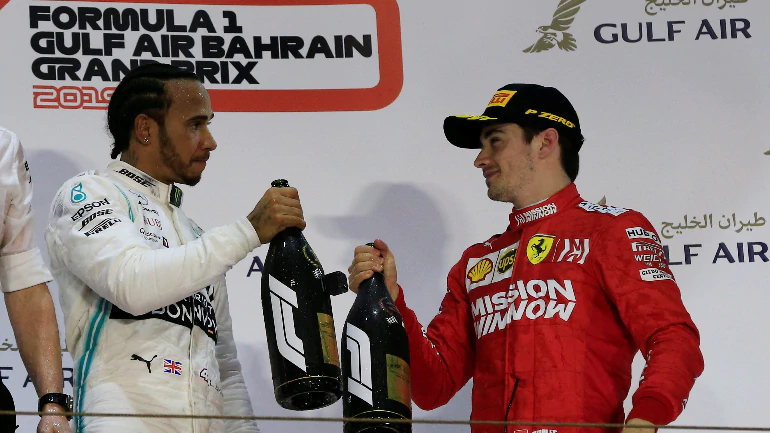
\includegraphics[width=1.00\textwidth]{pictures/charles_leclerc_champagne.jpg}
			Looking back on this module and this course, we feel like Charles Leclerc, 
			but maybe a bit more like he felt on Saturday than he did on the podium.
			We've pushed hard and done our best, but we ate the wall more than once.
			
			We will conclude with a page from the playbook of all the best drivers, 
			who always thank their team at the end of the race.
			We give our sincere thanks to the course staff and the team at Odyssey 
			for sharing their knowledge and responding to our questions at all hours.
			
			\textbf{ "Grazie mille, grazie ragazzi."}

%% bibliography

\begin{thebibliography}{9}
\bibitem{exo} 
Succi, Sauro: The Lattice Boltzmann Equation for Fluid Dynamics and Beyond

\end{thebibliography}

\end{document}


